\documentclass[paperwidth=47in,paperheight=71in,final, 16pt]{baposter}
%\setlength{\paperwidth}{47in} % A0 width: 46.8in
%\setlength{\textwidth}{22in}
%\setlength{\paperheight}{71in} % A0 height: 33.1in
%\setlength{\textwidth}{28in}
%below s added
%\documentclass[final, 12pt]{beamer}
%\documentclass[a4shrink,portrait,final]{baposter}
% Usa a4shrink for an a4 sized paper.

%\tracingstats=2

\usepackage{epsfig}
\usepackage{times}
\usepackage{calc}
\usepackage{graphicx}
\usepackage{amsmath}
\usepackage{amssymb}
\usepackage{relsize}
\usepackage{multirow}
\usepackage{bm}
\usepackage{enumitem}
\usepackage{multicol}
\usepackage{relsize,url}
\usepackage{graphics}
%below is added
%\usepackage[size=custom,orientation=portrait,scale=1.4,width =90, height=90,debug]{beamerposter}
\usepackage{pgfbaselayers}
\pgfdeclarelayer{background}
\pgfdeclarelayer{foreground}
\pgfsetlayers{background,main,foreground}

\usepackage{helvet}
\usepackage{bookman}
%\usepackage{palatino}
\usepackage{array}
\newcolumntype{L}[1]{>{\raggedright\let\newline\\\arraybackslash\hspace{0pt}}m{#1}}
\newcolumntype{C}[1]{>{\centering\let\newline\\\arraybackslash\hspace{0pt}}m{#1}}
\newcolumntype{R}[1]{>{\raggedleft\let\newline\\\arraybackslash\hspace{0pt}}m{#1}}
% mine

\usepackage{arydshln}
\usepackage{xspace,url,relsize}
\usepackage{mdwlist}

\newcommand{\corpus}[1]{\textsc{#1}\xspace}
\newcommand{\tool}[1]{\texttt{#1}\xspace}
\newcommand{\model}[1]{\textsc{#1}\xspace}

\newcommand{\topic}[1]{$\langle$\it#1$\rangle$}
\newcommand{\topiclabel}[1]{\textsc{#1}\xspace}
\newcommand{\dataset}[1]{\textsc{#1}\xspace}
\newcommand{\books}{\dataset{Books}}
\newcommand{\news}{\dataset{News}}
\newcommand{\blogs}{\dataset{Blogs}}
\newcommand{\pubmed}{\dataset{PubMed}}

\newcommand{\mymethod}[1]{\textsc{#1}\xspace}
\newcommand{\RACO}{\mymethod{raco}}

\newcounter{featcounter}
\newenvironment{featlist}{\begin{list}{\arabic{featcounter}.}{\usecounter{featcounter}}}{\end{list}}


\newsavebox{\fmbox}
\newenvironment{fmpage}[1]
{\begin{lrbox}{\fmbox}\begin{minipage}{#1}}
{\end{minipage}\end{lrbox}\fbox{\usebox{\fmbox}}}
% end mine

%\newcommand{\captionfont}{\footnotesize}

\selectcolormodel{cmyk}

\graphicspath{{img/}}

%%%%%%%%%%%%%%%%%%%%%%%%%%%%%%%%%%%%%%%%%%%%%%%%%%%%%%%%%%%%%%%%%%%%%%%%%%%%%%%%
%%%% Some math symbols used in the text
%%%%%%%%%%%%%%%%%%%%%%%%%%%%%%%%%%%%%%%%%%%%%%%%%%%%%%%%%%%%%%%%%%%%%%%%%%%%%%%%
% Format 
\newcommand{\Matrix}[1]{\begin{bmatrix} #1 \end{bmatrix}}
\newcommand{\Vector}[1]{\Matrix{#1}}
\newcommand*{\SET}[1]  {\ensuremath{\mathcal{#1}}}
\newcommand*{\MAT}[1]  {\ensuremath{\mathbf{#1}}}
\newcommand*{\VEC}[1]  {\ensuremath{\bm{#1}}}
\newcommand*{\CONST}[1]{\ensuremath{\mathit{#1}}}
\newcommand*{\norm}[1]{\mathopen\| #1 \mathclose\|}% use instead of $\|x\|$
\newcommand*{\abs}[1]{\mathopen| #1 \mathclose|}% use instead of $\|x\|$
\newcommand*{\absLR}[1]{\left| #1 \right|}% use instead of $\|x\|$
\newcommand{\spadeaff}{\ensuremath{\spadesuit}\xspace}
\newcommand{\clubaff}{\ensuremath{\clubsuit}\xspace}
\newcommand{\heartaff}{\ensuremath{\heartsuit}\xspace}
\newcommand{\diamondaff}{\ensuremath{\diamondsuit}\xspace}

\def\norm#1{\mathopen\| #1 \mathclose\|}% use instead of $\|x\|$
\newcommand{\normLR}[1]{\left\| #1 \right\|}% use instead of $\|x\|$

%%%%%%%%%%%%%%%%%%%%%%%%%%%%%%%%%%%%%%%%%%%%%%%%%%%%%%%%%%%%%%%%%%%%%%%%%%%%%%%%
% Multicol Settings
%%%%%%%%%%%%%%%%%%%%%%%%%%%%%%%%%%%%%%%%%%%%%%%%%%%%%%%%%%%%%%%%%%%%%%%%%%%%%%%%
\setlength{\columnsep}{0.7em}
\setlength{\columnseprule}{0mm}


%%%%%%%%%%%%%%%%%%%%%%%%%%%%%%%%%%%%%%%%%%%%%%%%%%%%%%%%%%%%%%%%%%%%%%%%%%%%%%%%
% Save space in lists. Use this after the opening of the list
%%%%%%%%%%%%%%%%%%%%%%%%%%%%%%%%%%%%%%%%%%%%%%%%%%%%%%%%%%%%%%%%%%%%%%%%%%%%%%%%
\newcommand{\compresslist}{%
\setlength{\itemsep}{0.2ex}%
\setlength{\parskip}{0.2ex}%
\setlength{\parsep}{0pt}%
}


%%%%%%%%%%%%%%%%%%%%%%%%%%%%%%%%%%%%%%%%%%%%%%%%%%%%%%%%%%%%%%%%%%%%%%%%%%%%%%
%%% Begin of Document
%%%%%%%%%%%%%%%%%%%%%%%%%%%%%%%%%%%%%%%%%%%%%%%%%%%%%%%%%%%%%%%%%%%%%%%%%%%%%%

\begin{document}

\larger
\sffamily

%%%%%%%%%%%%%%%%%%%%%%%%%%%%%%%%%%%%%%%%%%%%%%%%%%%%%%%%%%%%%%%%%%%%%%%%%%%%%%
%%% Here starts the poster
%%%---------------------------------------------------------------------------
%%% Format it to your taste with the options
%%%%%%%%%%%%%%%%%%%%%%%%%%%%%%%%%%%%%%%%%%%%%%%%%%%%%%%%%%%%%%%%%%%%%%%%%%%%%%
% Define some colors
\definecolor{silver}{cmyk}{0,0,0,0.3}
\definecolor{yellow}{cmyk}{0,0,0.9,0.0}
\definecolor{reddishyellow}{cmyk}{0,0.22,1.0,0.0}
\definecolor{black}{cmyk}{0,0,0.0,1.0}
\definecolor{darkYellow}{cmyk}{0,0,1.0,0.5}
\definecolor{darkSilver}{cmyk}{0,0,0,0.1}

\definecolor{darkGreen}{cmyk}{0.88,0,0.88,0.41}
\definecolor{midGreen}{cmyk}{0.71,0,0.66,0.01}

\definecolor{midBlue}{cmyk}{0.44,0.14,0,0.03}
\definecolor{lightSkyBlue}{cmyk}{0.31,0.11,0,0.00}
\definecolor{darkSkyBlue}{cmyk}{0.47,0.19,0,0.45}

\definecolor{darkRed}{cmyk}{0,1,1,0.56}
\definecolor{lightRed}{cmyk}{0,0.45,0.45,0.05}

\definecolor{myBlue}{rgb}{0.3,0.5,0.8}

%%
\typeout{Poster Starts}
\background{
  \begin{tikzpicture}[remember picture,overlay]%
    \draw (current page.north west)+(-20in,-20in) node[anchor=north west] {\includegraphics[height=1.1\textheight]{silhouettes_background}};
  \end{tikzpicture}%
}

\newlength{\leftimgwidth}
\begin{poster}%
  % Poster Options
  {
  % Show grid to help with alignment
  grid=no,
  % Column spacing
  colspacing=0.8em,
  columns=4,
  % Color style
  bgColorOne=white,
  bgColorTwo=white,
  borderColor=darkSkyBlue,
  %borderColor=silver,
  %headerColorOne=midBlue,
  headerColorOne=myBlue,
  headerColorTwo=reddishyellow,
  headerFontColor=black,
  boxColorOne=white,
  boxColorTwo=white,
  % Format of textbox
  textborder=rounded,
  % Format of text header
  eyecatcher=no,
  headerborder=open,
  headerheight=0.21\textheight,
  headershape=rounded,
  headershade=plain,
  %headerfont=\Large\textsf, %Sans Serif
  headerfont=\LARGE\textsc, %Sans Serif
textfont=\LARGE,
  boxshade=plain,
%  background=shade-tb,
  background=plain,
  linewidth=1pt
  }
  % Eye Catcher

  {
  }
  % Title
  %{\sf\LARGE\vspace*{2em}
  {
\Huge
\begin{tabular}{ccR{0.2cm}}
&  \bfseries Text-based Detection of Unauthorized Users of Social Media Accounts & \\
&\\
 & \textbf{Milton King, Dima Alhadidi, and Paul Cook}  & \\
 & \smaller University of New Brunswick & \\
\end{tabular}
 
    \vspace*{3ex}

  }
  % Authors

  {}


%%%%%%%%%%%%%%%%%%%%%%%%%%%%%%%%%%%%%%%%%%%%%%%%%%%%%%%%%%%%%%%%%%%%%%%%%%%%%%
  \headerbox{Author verification
}{name=verification,column=0,row=0,span=2}{
\vspace*{1ex}
%%%%%%%%%%%%%%%%%%%%%%%%%%%%%%%%%%%%%%%%%%%%%%%%%%%%%%%%%%%%%%%%%%%%%%%%%%%%%%
\begin{itemize}
\item Determine if a document is written by a specific known author
\item Models are trained on documents written by the known author
\item Unauthorized personnel can gain access to a social media account via the true user's devices or more advanced approaches
\item Imposters can publish potentially damaging information posing as the true owner of the account
\item Instances of damaging posts form imposters
\begin{itemize}

\item 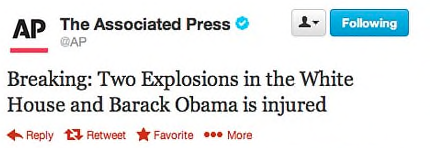
\includegraphics[width=0.8\linewidth]{./associatedPress.png}  \small{\\http://money.cnn.com/2017/03/16/technology/mcdonalds-trump-tweet/}
\LARGE
\item 
\includegraphics[width=0.8\linewidth]{./mcDonalds.png}
\small{\\http://www.telegraph.co.uk/finance/markets/10013768/Bogus-AP-tweet-about-explosion-at-the-White-House-wipes-billions-off-US-markets.html}


\end{itemize}
\end{itemize}
\vspace*{1ex}
}





%%%%%%%%%%%%%%%%%%%%%%%%%%%%%%%%%%%%%%%%%%%%%%%%%%%%%%%%%%%%%%%%%%%%%%%%%%%%%%
  \headerbox{Bench mark: Jankowska
}{name=jan,column=0,row=0,span=2,below=verification}{
\vspace*{1ex}
%%%%%%%%%%%%%%%%%%%%%%%%%%%%%%%%%%%%%%%%%%%%%%%%%%%%%%%%%%%%%%%%%%%%%%%%%%%%%%
\begin{itemize}

\item Label an unknown document as belonging to the known author if it is less dissimilar to all known documents than the most dissimilar known document is 
\vspace*{1ex}
\item \textbf{Original}: dissimilarity between two documents based on the differences in
frequencies of words in those documents.
\begin{equation*}\label{diff}
\mathit{diff} = {\sum_{x\in(D_1 \cup
    D_2)}{\left(\dfrac{fD_1(x)-fD_2(x)}{\frac{fD_1(x)+fD_2(x)}{2}}\right)}^2}
\end{equation*}
\vspace*{1ex}
\item \textbf{Vector compatible}: dissimilarity between two documents based on the cosine similarity of the vector representation of those documents.

\begin{center}
\begin{equation*}\label{diff}
\mathit{diff} ={Cos(V_i, V_k)}
\end{equation*}
\end{center}
\end{itemize}
\vspace*{2ex}


}


%%%%%%%%%%%%%%%%%%%%%%%%%%%%%%%%%%%%%%%%%%%%%%%%%%%%%%%%%%%%%%%%%%%%%%%%%%%%%%
  \headerbox{Models
}{name=models,column=2,row=0,span=2}{
%%%%%%%%%%%%%%%%%%%%%%%%%%%%%%%%%%%%%%%%%%%%%%%%%%%%%%%%%%%%%%%%%%%%%%%%%%%%%%
\begin{itemize}
\item Document representations
\begin{itemize}
\item Bag of words (BOW): Vector of word frequencies
\item Word2vec: Average word embeddings of words in the document
\begin{itemize}
\item Word2vec's Word embeddings: vector representations of words generated with an artificial neural network 
\end{itemize}
\end{itemize}

\item Classifiers
\begin{itemize}
\item Jankowska: Dissimilarity is measured by frequency of similar words
\item Augmented Jankowska: Dissimilarity measured by cosine similarity
\item One-class SVM: Trained on document representations
\end{itemize}

\end{itemize}

}

%%%%%%%%%%%%%%%%%%%%%%%%%%%%%%%%%%%%%%%%%%%%%%%%%%%%%%%%%%%%%%%%%%%%%%%%%%%%%%
  \headerbox{Datasets
}{name=eval,column=2,row=0,span=2, below=models}{
%%%%%%%%%%%%%%%%%%%%%%%%%%%%%%%%%%%%%%%%%%%%%%%%%%%%%%%%%%%%%%%%%%%%%%%%%%%%%%
\begin{itemize}

\item Total: 103 authors with more than 300 blog posts containing at least 100 words.

\item DEV: 10 authors with 90 test instances per author

\item TEST: 93 authors with 184 test instances per author


\item Classifiers are trained on documents belonging to the known author and then tested on a test set composed of half from the known author and one instance from each of the other authors in the dataset


\end{itemize}



}




%%%%%%%%%%%%%%%%%%%%%%%%%%%%%%%%%%%%%%%%%%%%%%%%%%%%%%%%%%%%%%%%%%%%%%%%%%%%%%
  \headerbox{Results
}{name=results,column=2,row=0,span=2, below=eval}{
%%%%%%%%%%%%%%%%%%%%%%%%%%%%%%%%%%%%%%%%%%%%%%%%%%%%%%%%%%%%%%%%%%%%%%%%%%%%%%
\large
\vspace*{1ex}

\begin{tabular}{|l|c|ccc|cccc|}
\hline

\multirow{2}{*}{Model} & \multirow{2}{*}{Acc} & \multicolumn{3}{|c|}{Negative} & \multicolumn{3}{|c|}{Positive} & \multirow{2}{*}{Avg. F}\\
\cline{3-8}
& & \multicolumn{1}{|c|}{P} & \multicolumn{1}{|c|}{R} & \multicolumn{1}{|c|}{F} & \multicolumn{1}{|c|}{P} & \multicolumn{1}{|c|}{R} & \multicolumn{1}{|c|}{F} & \\
\hline
All-in-one & \multicolumn{1}{|c|}{0.500} & \multicolumn{1}{|c|}{0.500} & \multicolumn{1}{|c|}{\textbf{1.00}} & \multicolumn{1}{|c|}{0.667} & \multicolumn{1}{|c|}{0} & \multicolumn{1}{|c|}{0} & \multicolumn{1}{|c|}{0} & \multicolumn{1}{|c|}{0.334}\\
Jan.& \multicolumn{1}{|c|}{0.516} &\multicolumn{1}{|c|}{0.534} & \multicolumn{1}{|c|}{0.764} &\multicolumn{1}{|c|}{0.566} &\multicolumn{1}{|c|}{0.268}&\multicolumn{1}{|c|}{0.268}& \multicolumn{1}{|c|}{0.228} & \multicolumn{1}{|c|}{0.397}\\
Jan.+BOW&\multicolumn{1}{|c|}{0.561}  &\multicolumn{1}{|c|}{0.552} & \multicolumn{1}{|c|}{0.912}&\multicolumn{1}{|c|}{\textbf{0.677}} & \multicolumn{1}{|c|}{0.518}&\multicolumn{1}{|c|}{0.211} & \multicolumn{1}{|c|}{0.255} & \multicolumn{1}{|c|}{0.466}\\
Jan.+word2vec&\multicolumn{1}{|c|}{0.576} &\multicolumn{1}{|c|}{\textbf{0.606}} &\multicolumn{1}{|c|}{0.542} &\multicolumn{1}{|c|}{0.529} &\multicolumn{1}{|c|}{0.595}&\multicolumn{1}{|c|}{\textbf{0.610}} & \multicolumn{1}{|c|}{\textbf{0.556}} &\multicolumn{1}{|c|}{0.543} \\
SVM+BOW &\multicolumn{1}{|c|}{0.566} &\multicolumn{1}{|c|}{0.557} &\multicolumn{1}{|c|}{0.613} & \multicolumn{1}{|c|}{0.582}& \multicolumn{1}{|c|}{0.582}& \multicolumn{1}{|c|}{0.519} & \multicolumn{1}{|c|}{0.545} & \multicolumn{1}{|c|}{0.564}\\
SVM+word2vec&\multicolumn{1}{|c|}{\textbf{0.594}}  &\multicolumn{1}{|c|}{0.567} &\multicolumn{1}{|c|}{0.704} &\multicolumn{1}{|c|}{0.625}& \multicolumn{1}{|c|}{\textbf{0.653}}& \multicolumn{1}{|c|}{0.484} & \multicolumn{1}{|c|}{0.547} & \multicolumn{1}{|c|}{\textbf{0.586}}\\
\hline
\end{tabular}

\vspace*{2ex}

}





%%%%%%%%%%%%%%%%%%%%%%%%%%%%%%%%%%%%%%%%%%%%%%%%%%%%%%%%%%%%%%%%%%%%%%%%%%%%%%
  \headerbox{Conclusions and Future Work
}{name=conclusion,column=2,row=0,span=2,below=results,bottomaligned=jan}{
%%%%%%%%%%%%%%%%%%%%%%%%%%%%%%%%%%%%%%%%%%%%%%%%%%%%%%%%%%%%%%%%%%%%%%%%%%%%%%

\begin{itemize}

\item Conclusions
\begin{itemize}
\item SVM+wordvec outperformed other models tested in terms of accuracy and average F1
\item We showed that the word2vec representation can better capture the writing style of an author used for verification using two different types of classifiers

\end{itemize}

\item Future work
\begin{itemize}
\item Find other document represenations to improve performance such as doc2vec
\end{itemize}

\end{itemize}

}




\end{poster}%
\end{document}


%%% Local Variables: 
%%% mode: latex
%%% TeX-command-default: "Make"
%%% TeX-master: t
%%% End: 
